\documentclass[11pt,letterpaper]{article}
\usepackage[T1]{fontenc}
\usepackage[utf8]{inputenc}
\usepackage[spanish,english,es-tabla,es-noquoting,es-nodecimaldot]{babel}
\usepackage{newtxtext,newtxmath}
\renewcommand{\ttdefault}{lmtt}
\usepackage{amsmath}
\usepackage[locale=US]{siunitx}
\sisetup{group-separator={\,},group-minimum-digits=4,separate-uncertainty=true,output-decimal-marker={.}}
\usepackage{booktabs,graphicx,float,array,tabularx,longtable}
\usepackage[labelsep=period,font=small,labelfont=bf]{caption}
\usepackage[margin=2.4cm]{geometry}
\usepackage{xcolor}
\definecolor{navy}{HTML}{1F3B63}
\usepackage{titlesec}
\titleformat{\section}{\normalfont\Large\bfseries}{\thesection.}{0.6em}{}
\titleformat{\subsection}{\normalfont\large\bfseries}{\thesubsection}{0.6em}{}
\titlespacing*{\section}{0pt}{14pt}{6pt}
\titlespacing*{\subsection}{0pt}{10pt}{4pt}
\usepackage{enumitem}
\setlist{itemsep=1pt,topsep=3pt}
\setlist[itemize]{label=$\bullet$}
\usepackage{listings}
\lstset{language=Python,basicstyle=\ttfamily\footnotesize,breaklines=true,frame=single,rulecolor=\color{black!40},showstringspaces=false,columns=fullflexible,keepspaces=true,extendedchars=true,literate={á}{{\'a}}1 {é}{{\'e}}1 {í}{{\'i}}1 {ó}{{\'o}}1 {ú}{{\'u}}1 {ñ}{{\~n}}1}
\usepackage{fancyhdr}
\pagestyle{fancy}\fancyhf{}
\fancyhead[L]{\small Análisis espectral de Fourier para alertas sísmicas}
\fancyhead[R]{\small\thepage}
\renewcommand{\headrulewidth}{0.4pt}
\setlength{\headheight}{14pt}
\usepackage{csquotes}
\usepackage[style=apa,backend=biber]{biblatex}
\addbibresource{refs.bib}
\usepackage{hyperref}
\hypersetup{colorlinks,allcolors=black,urlcolor=navy}
\setlength{\parindent}{0pt}
\setlength{\parskip}{5pt}
\setcounter{tocdepth}{1}
\newcommand{\fuente}{Fuente: elaboración propia.}

\begin{document}
\selectlanguage{spanish}

% ================= PORTADA =================
\begin{titlepage}
\centering
{\large\bfseries Instituto Tecnológico y de Estudios Superiores de Monterrey\par}
\vspace{2pt}
{\large Campus Monterrey\par}
\vspace{1.2cm}
{\large Análisis de Métodos Matemáticos para la Física\par}
\vfill
{\color{navy}\rule{\textwidth}{1.2pt}}\par\vspace{0.6cm}
{\large\scshape Reporte de investigación\par}\vspace{0.3cm}
{\fontsize{24}{30}\selectfont\bfseries Análisis espectral de Fourier para alertas\\[4pt] de señales sísmicas inclusivas\par}
\vspace{0.5cm}
{\large Separación de la onda sísmica y del ruido ambiental. Del experimento controlado a 20 sismos reales de México y al prototipo \textit{Sismo o ruido}\par}
\vspace{0.6cm}
{\color{navy}\rule{\textwidth}{1.2pt}}\par
\vfill
{\large\bfseries Equipo\par}
\vspace{6pt}
\begin{tabular}{ll}
Mateo Rodolfo Flores Torres & A01783438\\
Víctor Manuel Sánchez Chávez & A01287522\\
Sofía Martínez Alanis & A01724528\\
\end{tabular}
\par\vspace{0.8cm}
{\large Profesor: Dr. Luis Miguel Méndez Díaz\par}
\vspace{4pt}
{\normalsize Expo Ingenierías, 28.ª edición · Investigación y desarrollo de propuestas de mejora\par}
\vspace{4pt}
{\normalsize Prototipo: \url{https://sismo-o-ruido.vercel.app}\par}
\vspace{1.0cm}
{\large Monterrey, Nuevo León, noviembre de 2026\par}
\end{titlepage}

% ================= RESUMEN =================
\section*{Resumen}
\addcontentsline{toc}{section}{Resumen}
Los sistemas de alerta temprana necesitan separar la onda de un sismo del ruido que siempre registran sus sensores. Este trabajo lo aborda en dos etapas. La primera es un experimento controlado con dos registros simplificados del USGS, uno con sismo y otro solo con ruido ambiental. La serie de Fourier del registro con sismo muestra que un armónico de \SI{4.2}{s} concentra el \SI{94.8}{\percent} de su variación. Una regresión trigonométrica da amplitudes de $0.365 \pm 0.021$ y $0.062 \pm 0.002$, un cociente de energía de $35 \pm 5$ y una longitud de onda de unos \SI{18}{km}. El experimento revela su propio límite. El periodo de \SI{4}{s} cae en la banda de los microsismos oceánicos, así que la frecuencia sola no basta. La segunda etapa lleva el método a 20 sismos reales de México, de 1993 a 2026, registrados en Ciudad Universitaria. Como estos registros son largos y no periódicos, se usa la transformada de Fourier por ventanas. El ruido se estima antes de la llegada de la onda P y se resta en cada frecuencia con sustracción espectral. La relación señal-ruido mejora en los 20 sismos, en promedio \SI{10.5}{dB}, unas 11 veces en potencia. Con ruido real tan fuerte como el sismo, la correlación con la onda verdadera sube de 0.71 a 0.86. Los resultados se pueden explorar en el prototipo web \textit{Sismo o ruido}.

\textbf{Palabras clave:} serie de Fourier, transformada de Fourier de tiempo corto, sustracción espectral, ruido sísmico, alerta temprana.

\begin{otherlanguage}{english}
\section*{Abstract}
\addcontentsline{toc}{section}{Abstract}
Earthquake early warning systems must separate the earthquake wave from the noise their sensors always record. This work addresses the problem in two stages. The first is a controlled experiment with two simplified USGS records, one with an earthquake and one with ambient noise only. The Fourier series of the earthquake record shows that a \SI{4.2}{s} harmonic holds \SI{94.8}{\percent} of its variation. A trigonometric regression gives amplitudes of $0.365 \pm 0.021$ and $0.062 \pm 0.002$, an energy ratio of $35 \pm 5$ and a wavelength of about \SI{18}{km}. The experiment reveals its own limit, since the \SI{4}{s} period lies in the oceanic microseism band and frequency alone is not enough. The second stage extends the method to 20 real Mexican earthquakes from 1993 to 2026 recorded at Ciudad Universitaria. Because these records are long and non-periodic, a short-time Fourier transform is used. Noise is estimated before the P-wave arrival and removed at each frequency by spectral subtraction. The signal-to-noise ratio improves for all 20 earthquakes, by \SI{10.5}{dB} on average, about 11 times in power. With real noise as strong as the earthquake, the correlation with the true wave rises from 0.71 to 0.86. The results can be explored in the web prototype \textit{Sismo o ruido}.

\textbf{Keywords:} Fourier series, short-time Fourier transform, spectral subtraction, seismic noise, early warning.
\end{otherlanguage}

\clearpage
\tableofcontents
\clearpage

% ================= 1 INTRODUCCIÓN =================
\section{Introducción}
Los sismos están entre los riesgos naturales más letales. Varios terremotos del último siglo causaron más de \num{150000} muertes cada uno \parencite{statista2025}. La alerta temprana reduce el daño. Detecta las primeras ondas de un sismo y avisa antes de que lleguen las sacudidas fuertes \parencite{allen2019}. México opera el SASMEX desde 1991, el primer sistema público de alerta sísmica del mundo \parencite{espinosa1995}, y Estados Unidos opera ShakeAlert \parencite{usgs_ehp}.

El punto débil de estos sistemas es el ruido. Todas las estaciones registran vibraciones que no vienen del sismo, como el oleaje, el viento y la actividad humana \parencite{peterson1993,mcnamara2004}. Un sensor mide la suma de ambas partes y el sistema solo conoce esa suma. Si confunde ruido con sismo, da una falsa alarma. Si el ruido tapa la onda P, el aviso llega tarde. El tiempo de aviso ya es de pocos segundos cerca del epicentro \parencite{minson2018}, así que cada mejora en la detección importa.

Este problema no afecta a todos por igual. Las zonas rurales tienen menos sensores y reciben la alerta más tarde. Un método ligero, que corra en equipos de bajo costo, ayuda a cerrar esa brecha. Una alerta inclusiva también suma canales, como los altavoces del SASMEX \parencite{sasmex} o avisos visuales para personas sordas, y la población solo la sigue si confía en ella \parencite{allen2018eos}. Por eso el proyecto apoya el ODS~11, ciudades seguras y resilientes \parencite{onu11}, y el ODS~9, innovación en infraestructura \parencite{onu9}.

El trabajo responde dos preguntas, una por etapa.
\begin{enumerate}
\item \textit{Experimento controlado.} ¿Qué parte de un registro sísmico simplificado corresponde a la onda del sismo y qué parte puede explicarse por el ruido ambiental, si ambos se analizan con una serie de Fourier y una regresión trigonométrica?
\item \textit{Expansión a datos reales.} ¿Cuánto mejora la relación señal-ruido de un registro sísmico real si el ruido se estima antes de la onda P y se resta en cada frecuencia con la transformada de Fourier?
\end{enumerate}
La sección~2 fija los objetivos y las hipótesis. La sección~3 resume la teoría. La sección~4 describe el método en sus dos etapas y la sección~5 presenta los resultados en el mismo orden. Las secciones~6 y 7 discuten y concluyen.

% ================= 2 OBJETIVOS =================
\section{Objetivos, hipótesis y alcance}
\textbf{Objetivo general.} Separar la onda de un sismo del ruido ambiental con la serie y la transformada de Fourier, primero en un experimento controlado y después en 20 sismos reales de México, y poner el resultado al alcance de cualquier persona en un prototipo web.

\textbf{Objetivos específicos.}
\begin{enumerate}
\item Calcular la serie de Fourier y ajustar una regresión trigonométrica a los dos registros del USGS para obtener amplitud, fase, cociente de energía y longitud de onda.
\item Extender el método a registros reales con la transformada de Fourier por ventanas y la sustracción espectral, y medir la mejora de la relación señal-ruido.
\item Validar el método con un sismo sintético y con ruido real a distintos niveles.
\item Publicar un prototipo web que muestre la separación de cada sismo.
\end{enumerate}

\textbf{Hipótesis 1.} La componente dominante del registro con sismo tiene mucha más energía que la del registro de ruido. Durante un sismo el suelo se mueve mucho más que en reposo, y la energía crece con el cuadrado de la amplitud.

\textbf{Hipótesis 2.} En registros reales, restar el ruido estimado antes de la onda P aumenta la relación señal-ruido en todos los sismos analizados. El ruido de una estación cambia poco en unos minutos \parencite{mcnamara2004}, así que su espectro previo representa bien al que sigue presente durante el sismo.

\textbf{Alcance.} Se estudia la señal que registra un sensor, no el proceso del terremoto. La etapa 1 usa los dos registros simplificados del USGS \parencite{expediente}. La etapa 2 usa la componente vertical de una sola estación, G.UNM en Ciudad Universitaria \parencite{geoscope}, y 20 sismos de magnitud 6.8 o mayor del catálogo del USGS \parencite{comcat}. Quedan fuera la predicción de sismos, los modelos geológicos y la inteligencia artificial.

% ================= 3 MARCO TEÓRICO =================
\section{Marco teórico}

\subsection{Estado del arte}
La Tabla~\ref{tab:arte} resume los trabajos que sostienen este proyecto. Dejan tres ideas. El ruido tiene bandas conocidas, con un máximo oceánico entre 4 y \SI{8}{s} \parencite{peterson1993,longuet1950}. Los métodos actuales separan sismo y ruido usando a la vez el tiempo y la frecuencia \parencite{zhu2019,mousavi2016}. La sustracción espectral es una forma clásica y ligera de hacerlo \parencite{boll1979}.

\begin{table}[H]
\centering
\small
\begin{tabularx}{\textwidth}{>{\raggedright\arraybackslash}p{3.2cm}>{\raggedright\arraybackslash}p{3.3cm}X}
\toprule
Trabajo & Método & Hallazgo y relación con este proyecto\\
\midrule
\textcite{peterson1993} & Espectros de ruido de 75 estaciones & Modelos de ruido mínimo y máximo de la Tierra. Máximo entre 4 y 8 s.\\
\textcite{longuet1950} & Teoría de ondas oceánicas & El oleaje genera microsismos con periodos de 3 a 20 s.\\
\textcite{mcnamara2004} & Densidad espectral del ruido & El ruido cambia con la frecuencia, el sitio y la hora.\\
\textcite{brune1970} & Espectro de la fuente & Los sismos pequeños concentran su energía en frecuencias altas.\\
\textcite{boll1979} & Sustracción espectral & Estima el ruido cuando no hay señal y lo resta en cada frecuencia. Base de la etapa 2.\\
\textcite{berouti1979} & Sobresustracción y piso & Resta un poco más del ruido y limita la ganancia para evitar artefactos.\\
\textcite{mousavi2016} & Ruido en tiempo-frecuencia & Suprime ruido en registros sísmicos con la transformada de tiempo corto.\\
\textcite{zhu2019} & Redes neuronales & Separan sismo y ruido con una máscara tiempo-frecuencia. Estado actual del filtrado.\\
\textcite{minson2018} & Límites de la alerta & El aviso es corto cerca del epicentro. Cada segundo cuenta.\\
\bottomrule
\end{tabularx}
\caption{Estado del arte sobre ruido sísmico, separación de señales y alerta temprana.}
\label{tab:arte}
\end{table}

\subsection{Serie de Fourier y regresión trigonométrica}
Una señal periódica de periodo $T_0$ se escribe como una suma de ondas simples \parencite{fourier1822,kreyszig2011}:
\begin{equation}
x(t) = a_0 + \sum_{n=1}^{\infty}\left[a_n\cos(n\omega_0 t) + b_n\sin(n\omega_0 t)\right]
\label{eq:fourier}
\end{equation}
donde $\omega_0 = 2\pi/T_0$ en \si{rad/s} y $n$ es el número de armónico. Con $N$ datos tomados cada $\Delta t$, $T_0 = N\Delta t$ y los coeficientes son sumas:
\begin{equation}
a_0 = \frac{1}{N}\sum_{i=0}^{N-1} x_i, \qquad
a_n = \frac{2}{N}\sum_{i=0}^{N-1} x_i\cos(n\omega_0 t_i), \qquad
b_n = \frac{2}{N}\sum_{i=0}^{N-1} x_i\sin(n\omega_0 t_i)
\label{eq:coef}
\end{equation}
La frecuencia más alta observable es la de Nyquist, $f_{\max} = 1/(2\Delta t)$. Cada armónico es una onda de amplitud $A_n$ y fase $\varphi_n$, y su fracción de la varianza $\sigma^2$ sale del teorema de Parseval:
\begin{equation}
A_n = \sqrt{a_n^2 + b_n^2}, \qquad \varphi_n = \operatorname{atan2}(-b_n,\ a_n), \qquad p_n = \frac{A_n^2}{2\sigma^2}
\label{eq:Apn}
\end{equation}

Si un armónico domina, la señal se ajusta con una sola onda de frecuencia $\omega$ fija por mínimos cuadrados:
\begin{equation}
y(t) \approx c + a\cos(\omega t) + b\sin(\omega t), \qquad \left(\mathbf{M}^{T}\mathbf{M}\right)\boldsymbol{\beta} = \mathbf{M}^{T}\mathbf{y}
\label{eq:reg}
\end{equation}
donde cada fila de $\mathbf{M}$ es $(1, \cos\omega t_i, \sin\omega t_i)$ y $\boldsymbol{\beta} = (c, a, b)^T$. El error estándar de cada parámetro es $\mathrm{EE}(\beta_k) = s\sqrt{[(\mathbf{M}^T\mathbf{M})^{-1}]_{kk}}$, con $s^2 = S/(N-3)$ y $S$ la suma de los residuos al cuadrado.

\subsection{Onda, campos y energía}
El desplazamiento del suelo es un campo $\mathbf{u}(x,y,t)$. El sensor, fijo en un punto, registra su aceleración. La descomposición de Helmholtz separa el campo en una parte con divergencia, las ondas P, y una con rotacional, las ondas S \parencite{shearer2019}:
\begin{equation}
\mathbf{u} = \nabla\phi + \nabla\times\boldsymbol{\psi}, \qquad \nabla\cdot\mathbf{F} = \frac{\partial F_x}{\partial x} + \frac{\partial F_y}{\partial y}, \qquad \nabla\times\mathbf{F} = \frac{\partial F_y}{\partial x} - \frac{\partial F_x}{\partial y}
\label{eq:helm}
\end{equation}
Cada componente cumple la ecuación de onda con su velocidad $v$. Al sustituir una onda plana se obtiene la longitud de onda, y la energía media por unidad de volumen depende del cuadrado de la amplitud del desplazamiento $U$:
\begin{equation}
\frac{\partial^2 u}{\partial t^2} = v^2\nabla^2 u, \qquad \lambda = \frac{v}{f} = vT, \qquad \bar{e} = \frac{1}{2}\rho\,\omega^2 U^2
\label{eq:onda}
\end{equation}
donde $\rho$ es la densidad del medio en \si{kg/m^3}.

\subsection{De la serie a la transformada de Fourier}
La serie de Fourier supone que la señal se repite. Eso vale en un registro corto con casi dos ciclos completos, pero no en un registro sísmico real de varios minutos, donde el sismo empieza y termina. Una sola serie mezclaría el ruido de antes con el sismo de después. Para registros largos se usa la transformada de Fourier discreta en ventanas cortas. La transformada de $N$ datos es \parencite{cooley1965}:
\begin{equation}
X_k = \sum_{i=0}^{N-1} x_i\, e^{-\,i\,2\pi k i/N}, \qquad a_0 = \frac{X_0}{N}, \quad a_k = \frac{2}{N}\operatorname{Re}X_k, \quad b_k = -\frac{2}{N}\operatorname{Im}X_k
\label{eq:dft}
\end{equation}
La segunda parte de la Ec.~\eqref{eq:dft} muestra que la transformada da los mismos coeficientes que la Ec.~\eqref{eq:coef}. No es otro método. Es la misma serie calculada con un algoritmo rápido. La transformada de tiempo corto la aplica a ventanas de $L$ datos que avanzan $H$ datos cada vez:
\begin{equation}
X(m,k) = \sum_{i=0}^{L-1} x_{i+mH}\, w_i\, e^{-\,i\,2\pi k i/L}
\label{eq:stft}
\end{equation}
donde $m$ numera la ventana y $w_i$ es la ventana de Hann. Cada columna es una serie de Fourier corta. El mapa de $|X(m,k)|^2$ es el espectrograma.

\subsection{Ruido en el espectro y sustracción espectral}
Si el sismo $s$ y el ruido $r$ no están correlacionados, en promedio sus potencias se suman en cada celda, $|X|^2 \approx |S|^2 + |R|^2$. El ruido sube el piso del espectro, pero no parejo, porque tiene bandas propias. De ahí salen dos criterios. Si el sismo y el ruido ocupan frecuencias distintas, basta un filtro de banda. Si las comparten, hace falta usar también el tiempo.

La sustracción espectral usa el tiempo \parencite{boll1979}. Antes de la onda P solo hay ruido. Con las $M$ ventanas de esa zona se estima su potencia en cada frecuencia y cada celda se multiplica por una ganancia entre 0 y 1 \parencite{berouti1979}:
\begin{equation}
P_R(k) = \frac{1}{M}\sum_{m\,\in\,\text{ruido}} |X(m,k)|^2, \qquad G(m,k) = \sqrt{\max\!\left(1 - \beta\,\frac{P_R(k)}{|X(m,k)|^2},\ g_{\min}^2\right)}
\label{eq:ganancia}
\end{equation}
donde $\beta$ es la sobresustracción y $g_{\min}$ el piso espectral. La señal limpia es $G\,X$, se regresa al tiempo con la transformada inversa y el ruido estimado es la diferencia con el registro. La ganancia es una máscara, como en \textcite{zhu2019}, pero sale de una fórmula cerrada. La calidad se mide con la relación señal-ruido:
\begin{equation}
\mathrm{SNR} = 10\log_{10}\frac{\overline{s^2}_{\text{sismo}}}{\overline{s^2}_{\text{ruido}}}
\label{eq:snr}
\end{equation}
donde $\overline{s^2}$ es la potencia media en la ventana del sismo o en la de ruido. Cada \SI{10}{dB} multiplican por 10 la potencia.

% ================= 4 METODOLOGÍA =================
\section{Metodología}

\subsection{Enfoque en dos etapas}
La Figura~\ref{fig:enfoque} resume el enfoque. La etapa 1 prueba el razonamiento en un caso controlado, con pocos datos y una respuesta que se puede calcular a mano. Su resultado deja una pregunta abierta, porque el periodo dominante también es el del mar. La etapa 2 responde esa pregunta con registros reales y una herramienta que usa el tiempo además de la frecuencia. Después se valida y se publica en un prototipo.

\begin{figure}[H]
\centering
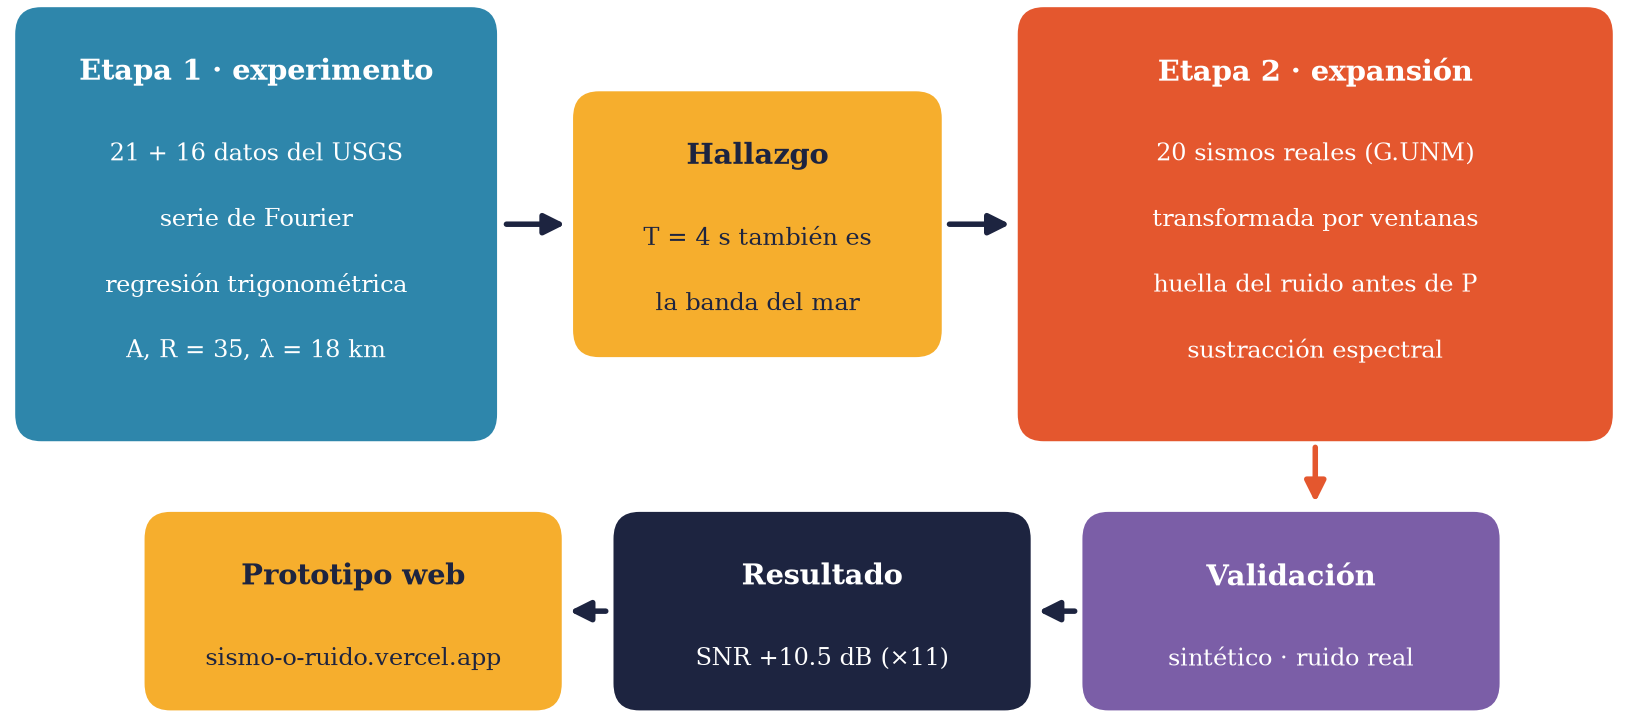
\includegraphics[width=0.95\textwidth]{enfoque.png}
\caption{Enfoque del proyecto. La etapa 1 prueba el método en un caso controlado y su límite motiva la etapa 2. \fuente}
\label{fig:enfoque}
\end{figure}

\subsection{Etapa 1 · experimento controlado}
\textbf{Datos.} Dos registros simplificados del USGS en aceleración normalizada, uno cada \SI{0.4}{s}. El del sensor tiene 21 datos durante un sismo y el ambiental 16 datos sin sismo (Tabla~\ref{tab:datos}). Los parámetros del medio son $\rho = \SI{2700}{kg/m^3}$ y $v = \SI{4500}{m/s}$ \parencite{expediente}.

\textbf{Supuestos.} Ambos registros usan la misma escala. El ambiental representa el ruido, aunque viene de otra estación y otro momento. Cada registro se describe con su componente dominante, ambos con el mismo periodo $T$, y la onda llega como onda plana a un medio homogéneo.

\textbf{Modelo.} El sensor mide la suma del sismo y del ruido, y cada registro se ajusta con la Ec.~\eqref{eq:reg}:
\begin{equation}
x(t) = s(t) + r(t), \qquad x_i \approx c_x + a_x\cos\omega t_i + b_x\sin\omega t_i, \qquad r_j \approx c_r + a_r\cos\omega t_j + b_r\sin\omega t_j
\label{eq:modelo}
\end{equation}
Como los datos son aceleraciones, $U = A/\omega^2$ y la energía de la Ec.~\eqref{eq:onda} queda $\bar e = \rho A^2/(2\omega^2)$. Al dividir la del sensor entre la del ruido se cancelan $\rho$ y $\omega$:
\begin{equation}
R = \frac{\bar e_x}{\bar e_r} = \left(\frac{A_x}{A_r}\right)^2, \qquad \frac{\delta R}{R} = 2\sqrt{\left(\frac{\delta A_x}{A_x}\right)^2 + \left(\frac{\delta A_r}{A_r}\right)^2}
\label{eq:R}
\end{equation}

\textbf{Procedimiento.} Se calculan los coeficientes con la Ec.~\eqref{eq:coef} y su peso con la Ec.~\eqref{eq:Apn} para hallar el armónico dominante. Se mide $T$ entre dos crestas y se resuelven las ecuaciones normales de cada registro. Con las amplitudes se calcula $R$ y con $T$ la longitud de onda $\lambda = vT$.

\begin{table}[H]
\centering
\small
\begin{tabular}{ccc@{\hspace{1.2cm}}ccc}
\toprule
$t$ (s) & Sensor & Ambiental & $t$ (s) & Sensor & Ambiental\\
\midrule
0.0 & 0.02 & 0.03 & 4.4 & $-0.04$ & 0.06\\
0.4 & 0.08 & 0.05 & 4.8 & 0.18 & 0.07\\
0.8 & 0.21 & 0.07 & 5.2 & 0.33 & 0.05\\
1.2 & 0.35 & 0.04 & 5.6 & 0.39 & 0.01\\
1.6 & 0.41 & 0.02 & 6.0 & 0.27 & $-0.03$\\
2.0 & 0.29 & $-0.01$ & 6.4 & 0.05 & --\\
2.4 & 0.10 & $-0.05$ & 6.8 & $-0.17$ & --\\
2.8 & $-0.12$ & $-0.06$ & 7.2 & $-0.34$ & --\\
3.2 & $-0.31$ & $-0.04$ & 7.6 & $-0.40$ & --\\
3.6 & $-0.38$ & $-0.01$ & 8.0 & $-0.22$ & --\\
4.0 & $-0.25$ & 0.03 & & & \\
\bottomrule
\end{tabular}
\caption{Registros simplificados del USGS en aceleración normalizada. Su límite de redondeo es $\pm 0.005$.}
\label{tab:datos}
\end{table}

\subsection{Etapa 2 · expansión a registros reales}
La etapa 2 repite la lógica de la etapa 1. Primero se mira el espectro, luego se separa y al final se valida. Cambian los datos y la herramienta. Todo está en el script \texttt{sismos\_fourier.py}, que usa ObsPy para descargar y preparar los datos \parencite{obspy2010}.
\begin{enumerate}
\item \textbf{Datos.} Se eligen 20 sismos conocidos de México con $M \geq 6.8$ y se descarga el canal vertical BHZ (20 muestras por segundo) de G.UNM desde EarthScope. Si una estación no tiene datos, el script busca otra del Servicio Sismológico Nacional \parencite{ssn}.
\item \textbf{Preparación.} Se corrige la respuesta del instrumento para obtener velocidad en \si{m/s}, se deja la banda de 0.04 a \SI{8}{Hz} y se recorta de 5 minutos antes a 10 minutos después de la onda P, calculada con el modelo iasp91.
\item \textbf{Espectrograma.} Se aplica la Ec.~\eqref{eq:stft} con ventanas de \SI{25.6}{s} (512 datos) y traslape de \SI{75}{\percent}. Esa ventana resuelve el pico de microsismos de 0.1 a \SI{0.35}{Hz}.
\item \textbf{Huella del ruido.} Se estima $P_R(k)$ con las ventanas que terminan \SI{40}{s} antes de la onda P. El margen evita que el sismo se cuele por el filtro y por la ventana.
\item \textbf{Resta.} Se aplica la Ec.~\eqref{eq:ganancia} con $\beta = 2$ y $g_{\min} = 0.02$, valores típicos de \textcite{berouti1979}, y la transformada inversa.
\item \textbf{Medición.} Se calcula la SNR en los 3 minutos después de la P y en sus primeros \SI{10}{s}, que son los que usa una alerta temprana.
\end{enumerate}

\subsection{Validación y prototipo}
El método se prueba de dos formas. La primera es un sismo sintético de forma conocida, sumado a ruido de microsismos. La segunda suma ruido real a cada sismo limpio a niveles de $-10$ a \SI{20}{dB}. Para alargar ese ruido se usan sustitutos de Fourier, que conservan su espectro y cambian sus fases al azar \parencite{theiler1992}. En ambos casos se compara la señal separada con la verdadera.

El prototipo \textit{Sismo o ruido} es una página web estática \parencite{prototipo}. El script exporta, por cada sismo, la señal cruda, el sismo y el ruido separados, sus espectros y sus espectrogramas. La página los dibuja en el navegador, sin servidor ni inteligencia artificial, y permite escuchar cada señal acelerada 400 veces \parencite{kilb2012}. Se publica en Vercel y su código está en GitHub.

\textbf{Herramientas y recursos.} Python 3 con NumPy, SciPy, Matplotlib y ObsPy, HTML y JavaScript para la web, y \LaTeX{} para el reporte. Todo es gratuito y corre en computadoras personales. Los datos vienen de los servidores públicos del USGS y de EarthScope. El equipo fueron tres estudiantes con la asesoría del profesor.

% ================= 5 RESULTADOS =================
\section{Resultados}

\subsection{Etapa 1 · experimento controlado}
Con los 21 datos del sensor, $T_0 = \SI{8.4}{s}$, $a_0 = 0.021$ y $f_{\max} = \SI{1.25}{Hz}$. La Tabla~\ref{tab:fourier} muestra que el segundo armónico, de periodo \SI{4.2}{s}, concentra el \SI{94.8}{\percent} de la variación. Eso justifica ajustar una sola onda. Los armónicos 7 a 10 aportan menos de \SI{0.1}{\percent} cada uno.

\begin{table}[H]
\centering
\small
\begin{tabular}{ccrrrcr}
\toprule
$n$ & $f_n$ (Hz) & $T_n$ (s) & $a_n$ & $b_n$ & $A_n$ & $p_n$ (\%)\\
\midrule
1 & 0.119 & 8.40 & 0.008 & 0.041 & 0.042 & 1.3\\
\textbf{2} & \textbf{0.238} & \textbf{4.20} & $\mathbf{-0.147}$ & \textbf{0.333} & \textbf{0.364} & \textbf{94.8}\\
3 & 0.357 & 2.80 & 0.047 & $-0.034$ & 0.058 & 2.4\\
4 & 0.476 & 2.10 & 0.031 & $-0.007$ & 0.031 & 0.7\\
5 & 0.595 & 1.68 & 0.018 & $-0.008$ & 0.019 & 0.3\\
6 & 0.714 & 1.40 & 0.024 & $-0.00049$ & 0.024 & 0.4\\
\bottomrule
\end{tabular}
\caption{Coeficientes de Fourier del registro del sensor.}
\label{tab:fourier}
\end{table}

\textit{Ejemplo de sustitución:} $a_2 = \frac{2}{21}\sum x_i\cos(2\omega_0 t_i) = \frac{2}{21}(-1.548) = -0.147$. La misma cifra sale de la Ec.~\eqref{eq:dft} con la transformada rápida.

La distancia entre crestas es de \SI{4.0}{s} en ambos registros, así que se fija $\omega = 2\pi/\SI{4.0}{s} = \SI{1.571}{rad/s}$. La Tabla~\ref{tab:ajuste} da los parámetros de la regresión. Las curvas explican el \SI{94.6}{\percent} de la variación del sensor y el \SI{98.3}{\percent} de la del ruido.

\begin{table}[H]
\centering
\small
\begin{tabular}{lcccccc}
\toprule
Registro & $c$ & $a$ & $b$ & $A$ & $\varphi$ (rad) & $R^2$\\
\midrule
Sensor & $0.033 \pm 0.015$ & $-0.237 \pm 0.020$ & $0.278 \pm 0.021$ & $0.365 \pm 0.021$ & $-2.28$ & 0.95\\
Ambiental & $0.004 \pm 0.002$ & $0.026 \pm 0.002$ & $0.056 \pm 0.002$ & $0.062 \pm 0.002$ & $-1.14$ & 0.98\\
\bottomrule
\end{tabular}
\caption{Regresión trigonométrica con $T = \SI{4.0}{s}$.}
\label{tab:ajuste}
\end{table}

\textit{Ejemplo de sustitución (sensor):} las ecuaciones normales son
$\begin{pmatrix} 21 & 1 & 0\\ 1 & 11 & 0\\ 0 & 0 & 10 \end{pmatrix}\boldsymbol{\beta} = \begin{pmatrix} 0.450\\ -2.578\\ 2.776 \end{pmatrix}$, de donde $b_x = 0.278$, $a_x = -0.237$, $c_x = 0.033$ y $A_x = 0.365$.

La amplitud del sensor es 5.92 veces la del ruido. Con la Ec.~\eqref{eq:R}, $R = (0.365/0.062)^2 = 35 \pm 5$ y la hipótesis 1 se cumple. La longitud de onda es $\lambda = (\SI{4500}{m/s})(\SI{4.0}{s}) \approx \SI{18000}{m}$, del orden de la profundidad de \SI{15}{km}. La Figura~\ref{fig:ajuste} muestra los ajustes.

\begin{figure}[H]
\centering
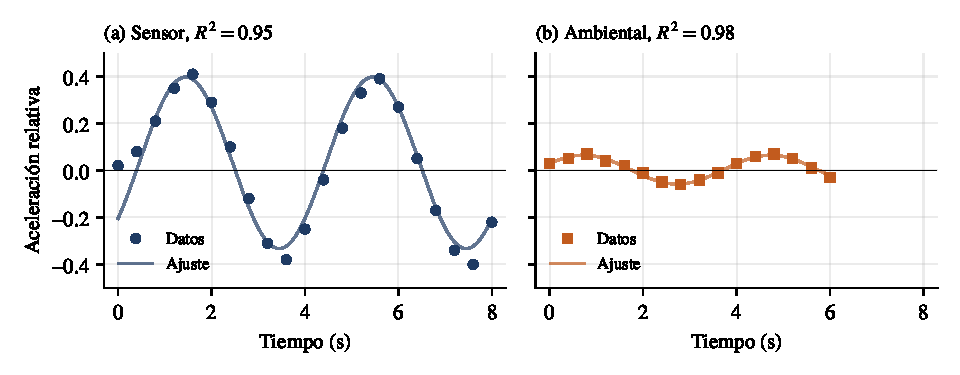
\includegraphics[width=0.82\textwidth]{ajuste.pdf}
\caption{Ajuste de una onda a cada registro del USGS. \fuente}
\label{fig:ajuste}
\end{figure}

\textbf{Lo que deja abierto la etapa 1.} Los dos registros tienen el mismo periodo de \SI{4}{s}, y ese periodo cae en la banda de los microsismos que produce el oleaje \parencite{longuet1950,peterson1993}. La diferencia aparece en la amplitud, no en la frecuencia. En datos reales, una componente de \SI{4}{s} podría ser mar y no sismo. Además, con un dato cada \SI{0.4}{s} no se ve nada por encima de \SI{1.25}{Hz}, donde está la energía de los sismos pequeños \parencite{brune1970}. Estas dos limitaciones son las que atiende la etapa 2.

\subsection{Etapa 2 · registros reales}
La Figura~\ref{fig:registro} muestra el sismo de Puebla-Morelos de 2017 visto desde Ciudad Universitaria, a \SI{113}{km} del epicentro. El registro crudo se separa en sismo y ruido. Antes de la onda P, el sismo separado queda casi en cero y el ruido conserva su forma.

\begin{figure}[H]
\centering
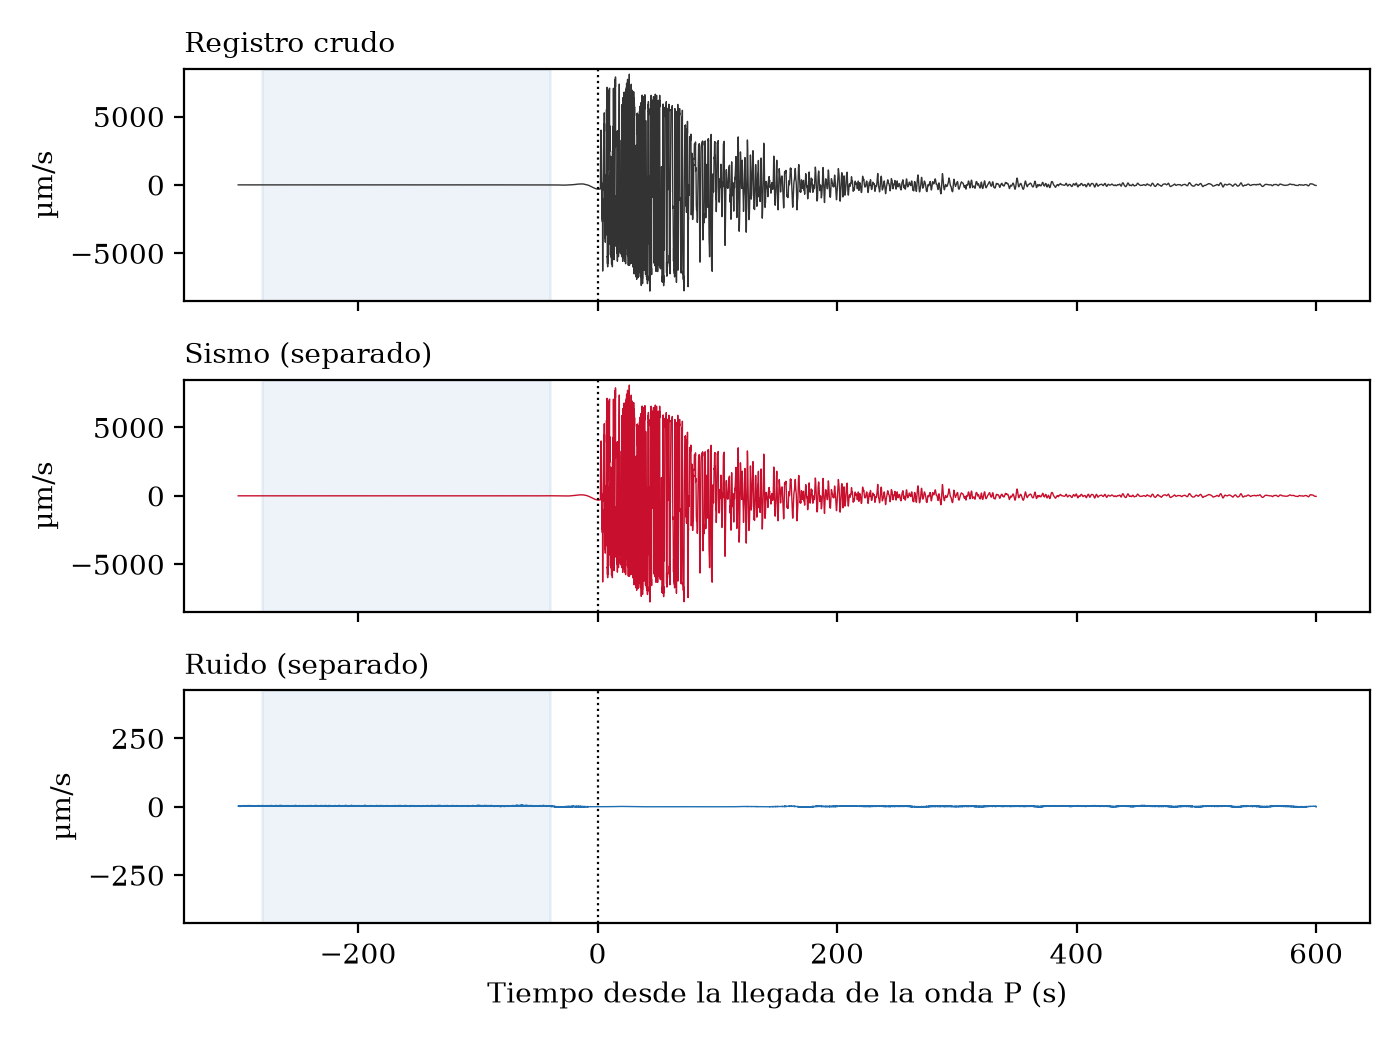
\includegraphics[width=0.85\textwidth]{real_registro.png}
\caption{Sismo de Puebla-Morelos (19 de septiembre de 2017, $M$ 7.1) en G.UNM. La franja azul es la ventana de ruido y el ruido separado se muestra amplificado. Fuente: elaboración propia con datos del USGS y EarthScope.}
\label{fig:registro}
\end{figure}

La Figura~\ref{fig:espectro} compara los espectros de la ventana del sismo y de la de ruido. El sismo está de 100 a \num{10000} veces por encima del ruido. La Figura~\ref{fig:peterson} ubica el ruido entre los modelos de \textcite{peterson1993}. Entre 3 y \SI{10}{s} aparece el pico de los microsismos, y por debajo de \SI{1}{s} el ruido urbano de la Ciudad de México rebasa el modelo de ruido alto. En los 20 sismos, el pico oceánico tiene una mediana de \SI{6.4}{s} (de 3.0 a \SI{9.6}{s}) y solo guarda el \SI{14}{\percent} de la energía del ruido. Esto confirma el límite de la etapa 1. El ruido real sí tiene energía en la banda de \SI{4}{s}.

\begin{figure}[H]
\centering
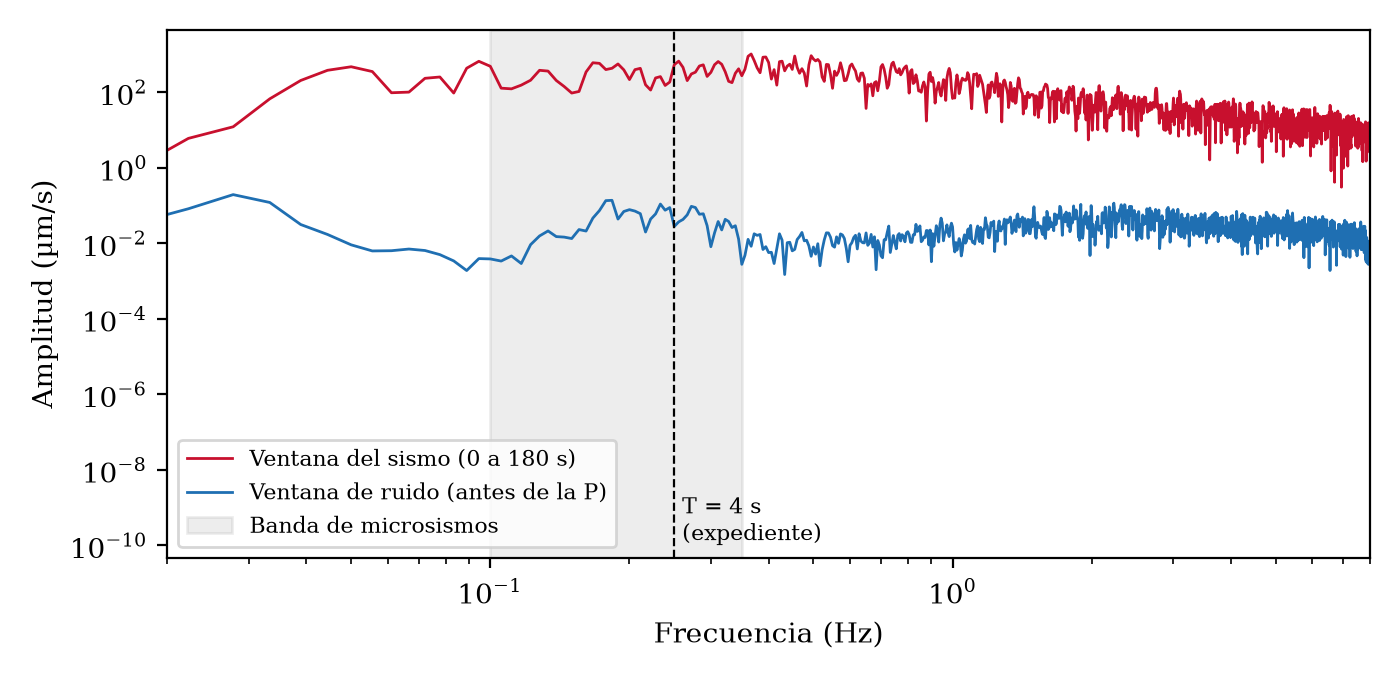
\includegraphics[width=0.85\textwidth]{real_espectro.png}
\caption{Espectro de amplitud del sismo de Puebla-Morelos y del ruido previo. La línea punteada marca el periodo de \SI{4}{s} de la etapa 1. \fuente}
\label{fig:espectro}
\end{figure}

\begin{figure}[H]
\centering
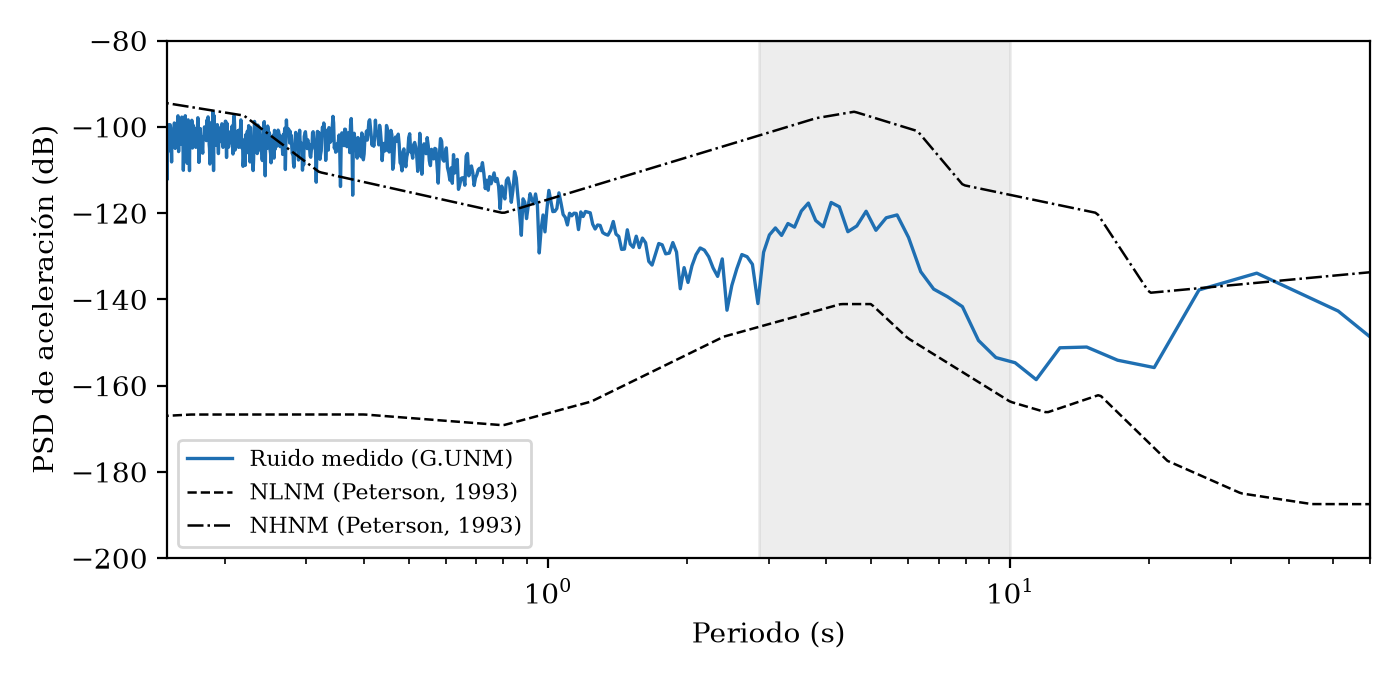
\includegraphics[width=0.85\textwidth]{real_peterson.png}
\caption{Densidad espectral del ruido de G.UNM, calculada con el método de \textcite{welch1967}, frente a los modelos de ruido mínimo (NLNM) y máximo (NHNM). La franja gris es la banda de microsismos. \fuente}
\label{fig:peterson}
\end{figure}

La Figura~\ref{fig:espectrograma} muestra el espectrograma antes y después de la resta. La zona previa a la onda P se apaga y el sismo queda igual. La Tabla~\ref{tab:sismos} y la Figura~\ref{fig:resumen} resumen los 20 sismos. La SNR subió en todos, de 3.3 a \SI{17.6}{dB}, con un promedio de \SI{10.5}{dB}. En los primeros \SI{10}{s} de la onda P la mejora promedio es de \SI{10.0}{dB}. La hipótesis 2 se cumple. El caso más difícil es el del Golfo de California de 2012. A \SI{1754}{km}, su onda P casi no se distingue del ruido.

\begin{figure}[H]
\centering
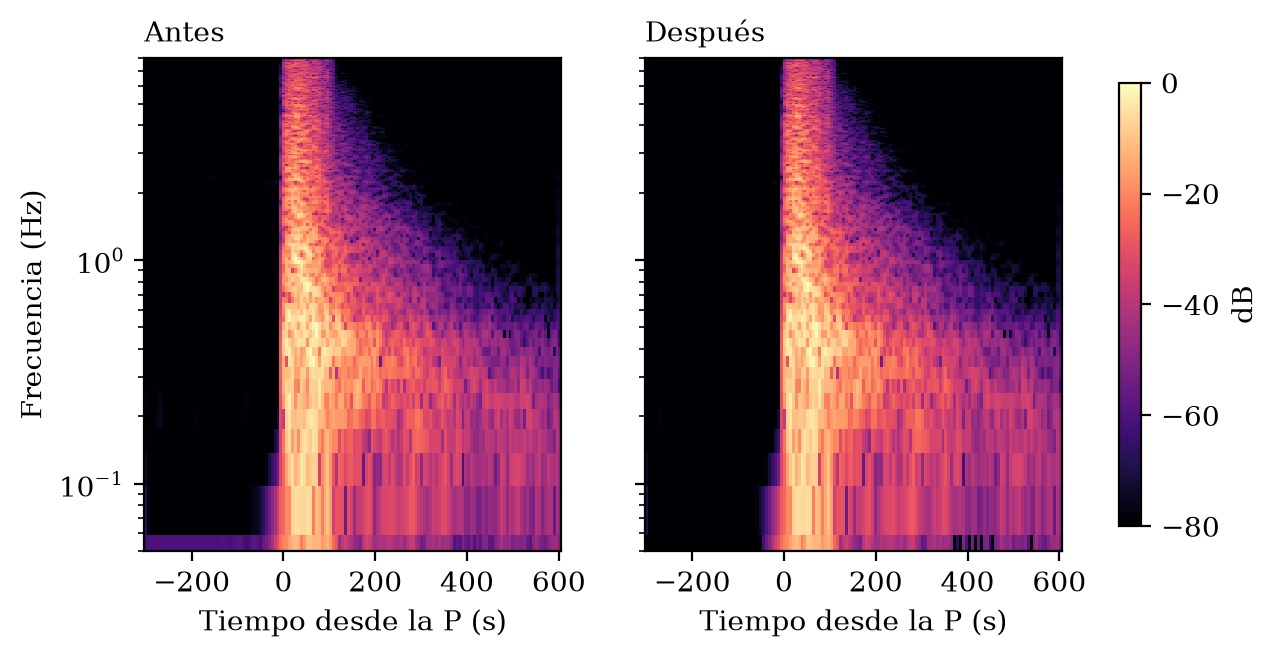
\includegraphics[width=0.85\textwidth]{real_espectrograma.png}
\caption{Espectrograma del sismo de Puebla-Morelos antes y después de la sustracción espectral. \fuente}
\label{fig:espectrograma}
\end{figure}

{\small\begin{longtable}{lcccccccc}
\toprule
Sismo & Fecha & $M$ & $d$ (km) & \multicolumn{2}{c}{SNR (dB)} & \multicolumn{2}{c}{SNR 10 s de P (dB)} & $T_{\text{mar}}$ (s)\\
\cmidrule(lr){5-6}\cmidrule(lr){7-8}
 & & & & antes & después & antes & después & \\
\midrule\endhead
Chiapas 1993 & 1993-09-10 & 7.2 & 863 & 39.8 & 50.0 & 13.3 & 22.9 & 9.6\\
Copala 1995 & 1995-09-14 & 7.4 & 289 & 61.5 & 76.4 & 43.1 & 58.1 & 3.9\\
Chiapas 1995 & 1995-10-21 & 7.2 & 664 & 50.6 & 61.7 & 35.6 & 46.6 & 5.6\\
Michoacán 1997 & 1997-01-11 & 7.2 & 397 & 66.3 & 74.5 & 41.2 & 49.4 & 4.4\\
Tehuacán 1999 & 1999-06-15 & 7.0 & 211 & 65.4 & 75.5 & 54.6 & 64.7 & 7.5\\
Oaxaca 1999 & 1999-09-30 & 7.5 & 433 & 47.8 & 58.8 & 36.5 & 47.6 & 3.5\\
Tecomán 2003 & 2003-01-22 & 7.6 & 522 & 67.0 & 77.2 & 39.5 & 49.7 & 6.9\\
El Mayor-Cucapah 2010 & 2010-04-04 & 7.2 & 2\,156 & 35.7 & 45.7 & 9.8 & 19.2 & 6.0\\
Ometepec 2012 & 2012-03-20 & 7.4 & 330 & 62.8 & 80.3 & 46.0 & 63.4 & 7.1\\
Golfo de California 2012 & 2012-04-12 & 7.0 & 1\,754 & 8.2 & 16.7 & -2.1 & -1.5 & 9.6\\
Papanoa 2014 & 2014-04-18 & 7.2 & 286 & 57.2 & 60.5 & 38.7 & 42.0 & 3.0\\
Chiapas 2014 & 2014-07-07 & 6.9 & 878 & 55.0 & 63.7 & 32.6 & 41.3 & 7.7\\
Tehuantepec 2017 & 2017-09-08 & 8.2 & 736 & 75.1 & 81.5 & 39.0 & 45.3 & 3.7\\
Puebla-Morelos 2017 & 2017-09-19 & 7.1 & 113 & 59.8 & 77.4 & 59.7 & 77.3 & 5.6\\
Pinotepa 2018 & 2018-02-16 & 7.2 & 350 & 64.5 & 76.7 & 39.6 & 51.8 & 6.7\\
Huatulco 2020 & 2020-06-23 & 7.4 & 508 & 68.0 & 81.4 & 42.4 & 55.7 & 7.5\\
Acapulco 2021 & 2021-09-08 & 7.0 & 271 & 72.8 & 80.3 & 59.2 & 66.7 & 7.3\\
Michoacán 2022 & 2022-09-19 & 7.6 & 410 & 68.2 & 78.9 & 28.7 & 39.4 & 8.0\\
Réplica Michoacán 2022 & 2022-09-22 & 6.8 & 415 & 71.9 & 80.1 & 45.9 & 54.2 & 6.2\\
Chiapas 2026 & 2026-07-17 & 7.3 & 846 & 45.6 & 55.2 & 22.4 & 31.9 & 6.0\\
\midrule
Promedio & & & & 57.2 & 67.6 & 36.3 & 46.3 & 6.4\textsuperscript{a}\\
\bottomrule
\caption{Resultados del método en los 20 sismos, registrados en la estación G.UNM. $d$ es la distancia epicentral y $T_{\text{mar}}$ el periodo del pico de microsismos del ruido. \textsuperscript{a}Mediana.}
\label{tab:sismos}
\end{longtable}}

\begin{figure}[H]
\centering
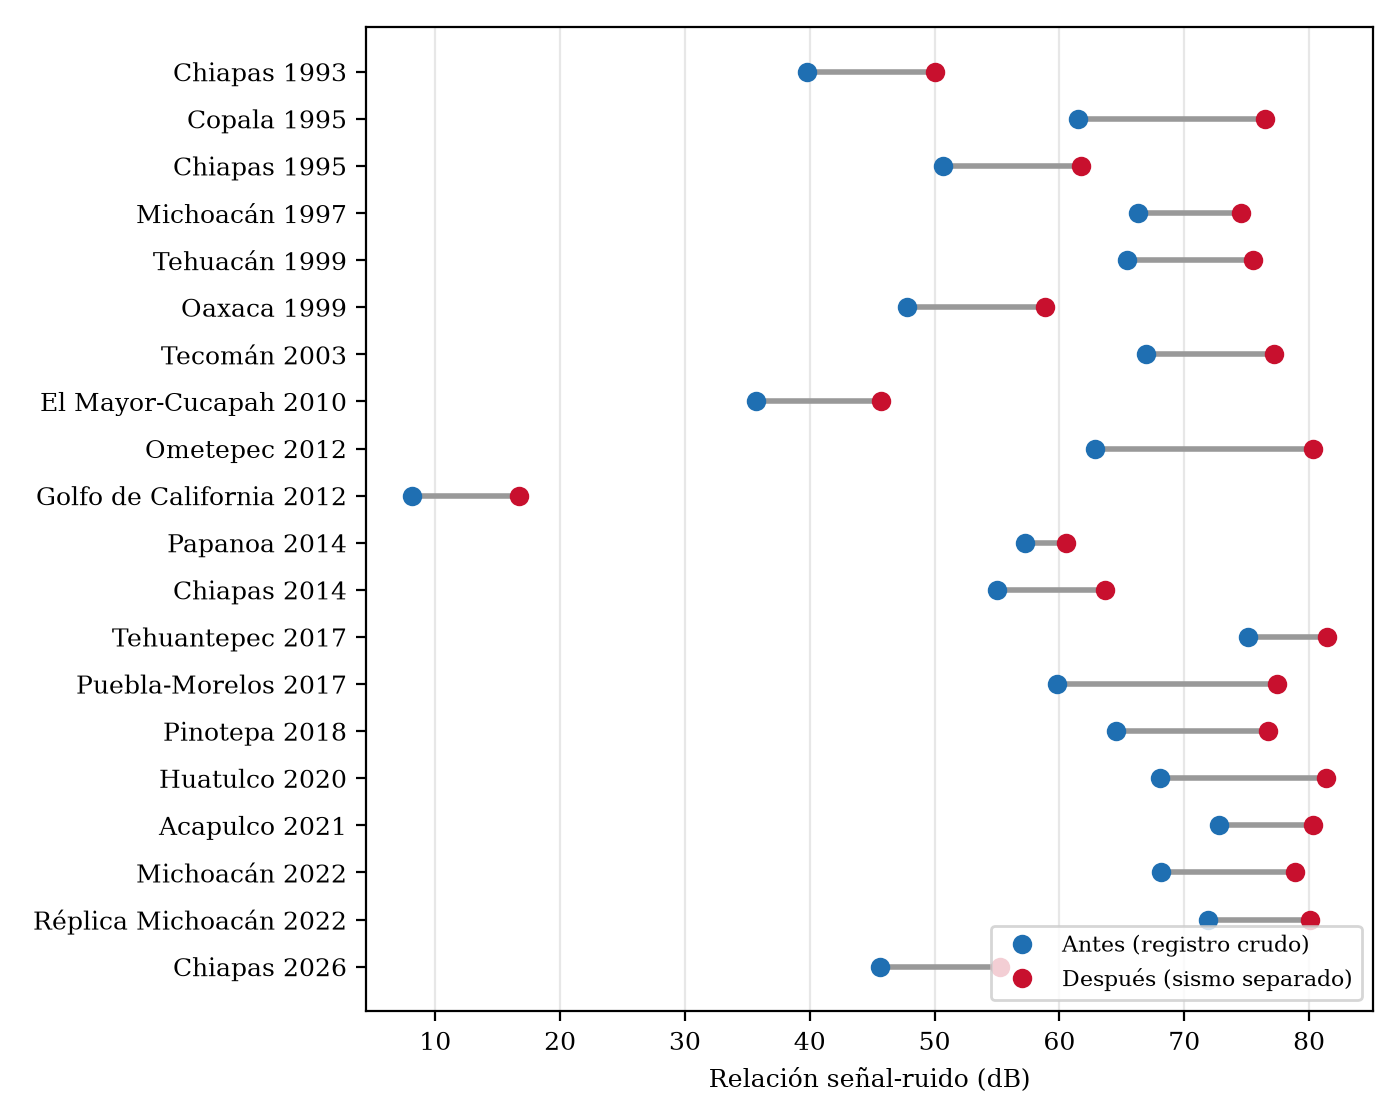
\includegraphics[width=0.78\textwidth]{real_resumen.png}
\caption{Relación señal-ruido de cada sismo antes y después de la sustracción espectral. \fuente}
\label{fig:resumen}
\end{figure}

\subsection{Validación}
La prueba sintética recupera el sismo conocido con una correlación de 0.996, y su SNR pasa de 5.9 a \SI{22.5}{dB}. La Figura~\ref{fig:robustez} muestra la prueba con ruido real. Con ruido tan fuerte como el sismo (\SI{0}{dB}), la correlación con la onda verdadera sube de 0.71 a 0.86. Con ruido tres veces más fuerte (\SI{-5}{dB}), sube de 0.48 a 0.67. Por encima de \SI{10}{dB}, el método no daña la señal.

\begin{figure}[H]
\centering
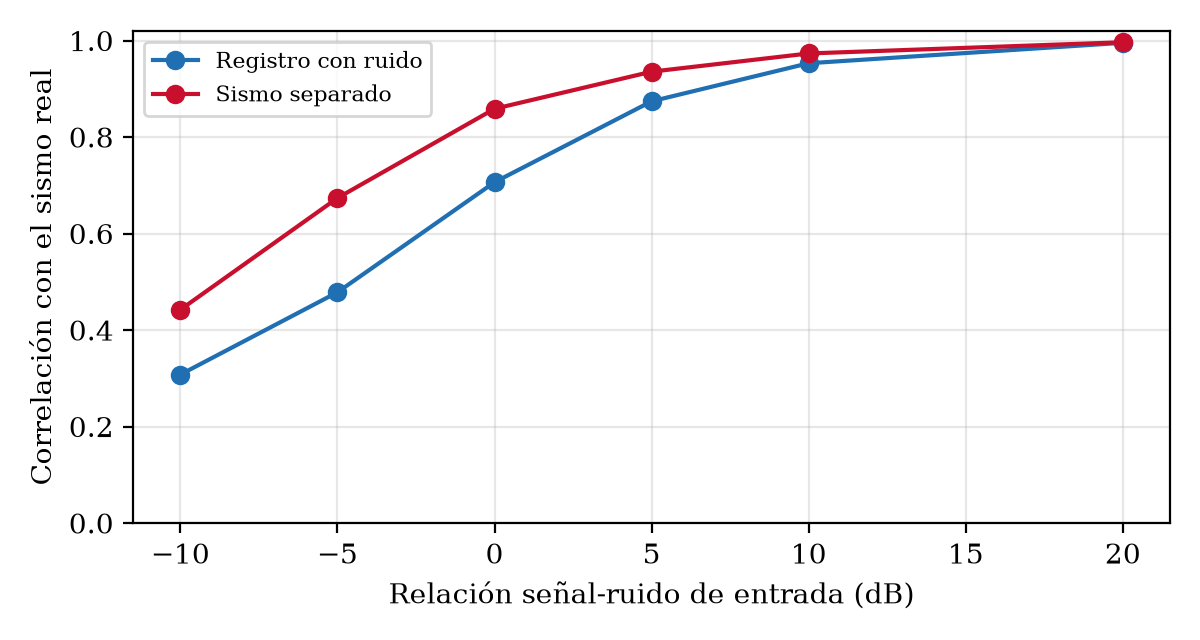
\includegraphics[width=0.72\textwidth]{real_robustez.png}
\caption{Correlación con el sismo real antes y después de separar, para distintos niveles de ruido real. Promedio de los 20 sismos. \fuente}
\label{fig:robustez}
\end{figure}

\subsection{Prototipo \textit{Sismo o ruido}}
El prototipo está en \url{https://sismo-o-ruido.vercel.app} y funciona en computadora y celular (Figura~\ref{fig:web}). La persona elige un sismo en el mapa. Con el botón \textit{Separar}, la señal se divide en sismo y ruido, y debajo aparecen sus frecuencias, el espectrograma antes y después y tres cifras clave. Usa los mismos datos de la Tabla~\ref{tab:sismos}, así que cualquiera puede revisar este reporte.

\begin{figure}[H]
\centering
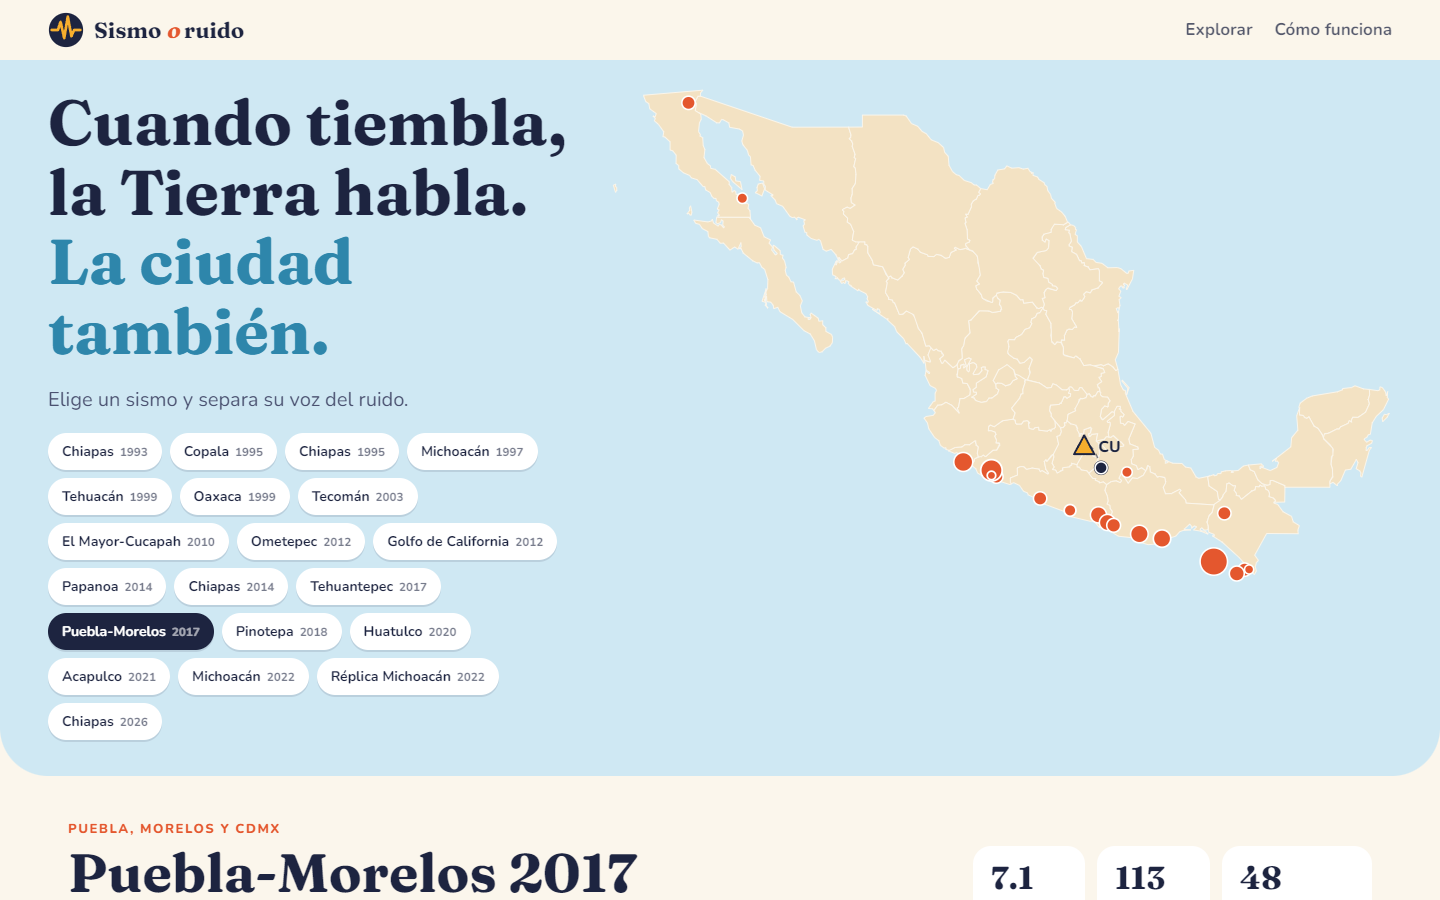
\includegraphics[width=0.49\textwidth]{web_portada.png}\hfill
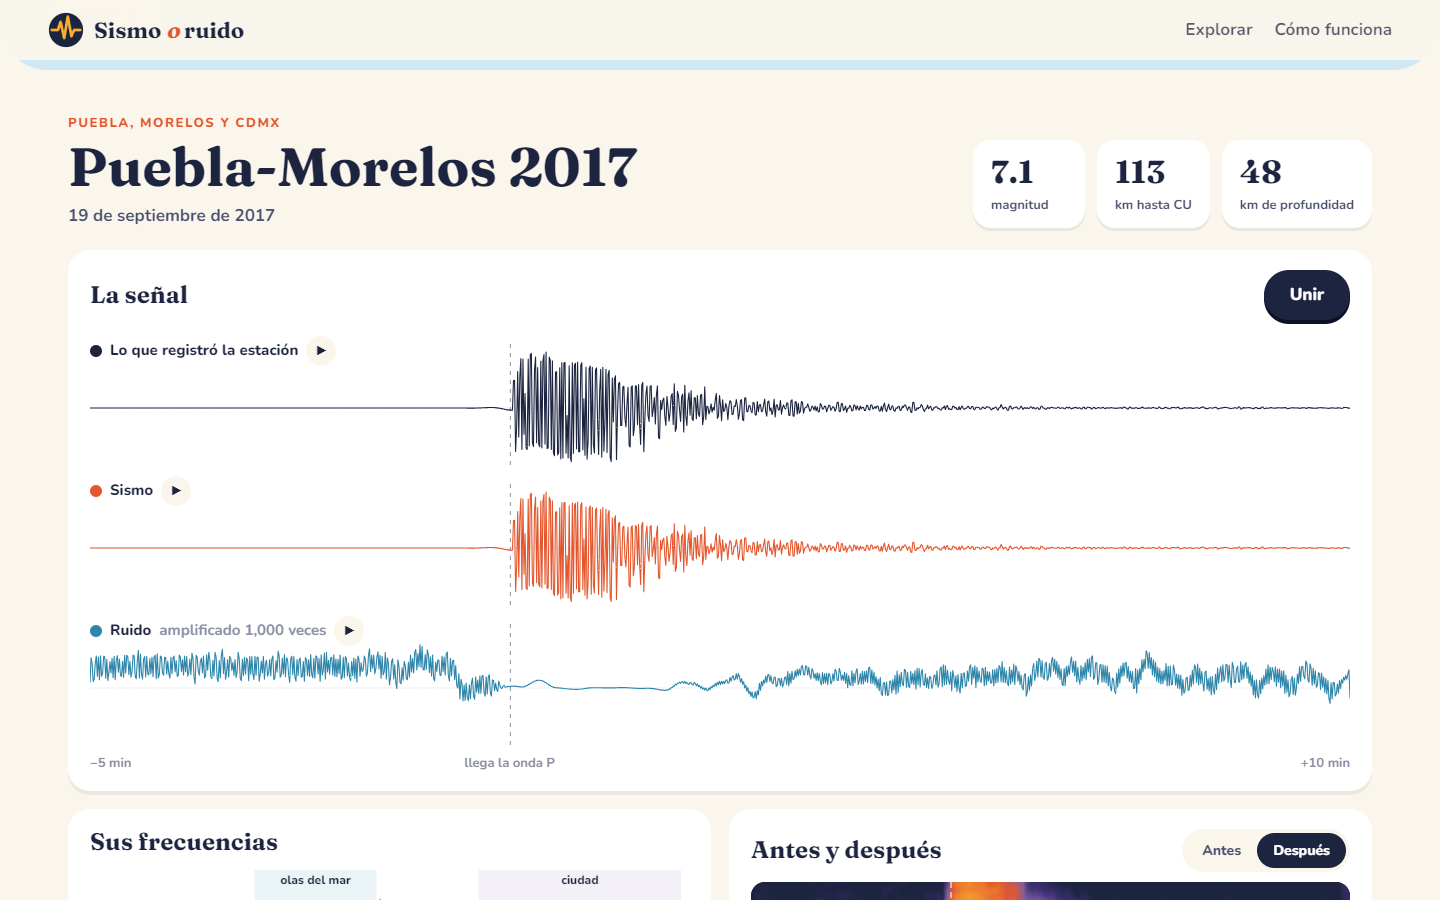
\includegraphics[width=0.49\textwidth]{web_ficha.png}
\caption{Prototipo \textit{Sismo o ruido}. A la izquierda, el mapa con los 20 sismos y la estación de CU. A la derecha, el sismo de Puebla-Morelos separado. \fuente}
\label{fig:web}
\end{figure}

% ================= 6 DISCUSIÓN =================
\section{Discusión}
\textbf{Las dos etapas se complementan.} La etapa 1 confirmó con números exactos que el sismo tiene unas 35 veces más energía que el ruido. Pero también mostró que esa diferencia está en la amplitud y no en la frecuencia. La etapa 2 confirmó con datos reales que el mar sí produce ruido en esa banda. Un filtro que solo mirara la frecuencia lo confundiría con un sismo. La sustracción espectral resuelve el problema porque usa el tiempo. Aprende el ruido antes de la onda P y lo resta después.

\textbf{Interpretación del cociente $R$.} El valor de 35 compara las componentes ajustadas bajo los supuestos del modelo. No dice qué porcentaje del sensor es sismo, porque el registro ambiental viene de otra estación y otro momento. En la etapa 2 esa limitación desaparece, porque el ruido se mide en la misma estación, minutos antes.

\textbf{Lectura física.} La longitud de onda de unos \SI{18}{km} es del orden de la profundidad de análisis. Con un solo sensor no se pueden medir variaciones espaciales, así que la separación en ondas P y S de la Ec.~\eqref{eq:helm} es teórica. En los registros reales sí se ve la llegada de la P y su uso como marca de tiempo.

\textbf{Lo que el método no hace.} Supone que el ruido no cambia durante el sismo. El ruido que llega mientras tiembla queda mezclado con el sismo, porque en esas celdas la señal es mucho mayor. Los 20 sismos son grandes y su SNR inicial ya es alta. El método aporta más en sismos pequeños o lejanos, como el del Golfo de California, que son justo los más difíciles.

% ================= 7 CONCLUSIONES =================
\section{Conclusiones}
\begin{itemize}
\item En el experimento controlado, un armónico de \SI{4.2}{s} explica el \SI{94.8}{\percent} de la señal. La regresión da un cociente de energía de $35 \pm 5$ y una longitud de onda de unos \SI{18}{km}.
\item El periodo de \SI{4}{s} coincide con el ruido del mar, así que la frecuencia sola no separa sismo y ruido. Ese límite motivó la segunda etapa.
\item La transformada de Fourier es la misma serie calculada en ventanas. Con ella y con la sustracción espectral, la relación señal-ruido mejoró en los 20 sismos reales, en promedio \SI{10.5}{dB}.
\item El método es robusto. Con ruido tan fuerte como el sismo, la correlación con la onda real sube de 0.71 a 0.86.
\item El prototipo \textit{Sismo o ruido} hace estos resultados accesibles, gratis y sin conocimientos previos.
\end{itemize}

\textbf{Impacto.} El método no necesita entrenar modelos ni equipo caro y corre en segundos en una computadora común. Puede servir como primer filtro en estaciones con poca capacidad de cómputo, que suelen estar en zonas rurales. El prototipo acerca la ciencia de la alerta sísmica a estudiantes y a la población, y la confianza en la alerta crece cuando la gente entiende cómo funciona \parencite{allen2018eos}.

\textbf{Limitaciones y trabajo futuro.} La etapa 1 usa registros cortos, de otra estación y con muestreo grueso. La etapa 2 usa una sola estación, una componente y sismos grandes. Conviene probar el método con sismos pequeños, con varias estaciones y con un ruido que se actualice durante el registro, como en \textcite{mousavi2016}.

% ================= BIBLIOGRAFÍA =================
\printbibliography[title={Referencias}]

% ================= ANEXO =================
\appendix
\section*{Anexo. Código}
\addcontentsline{toc}{section}{Anexo. Código}
El siguiente código reproduce los resultados de la etapa 1. El script de la etapa 2, \texttt{sismos\_fourier.py}, descarga los 20 sismos, aplica el método, hace las pruebas y exporta las figuras y los datos del prototipo. Está completo en \url{https://github.com/Mmateo101/video-fismat}.
\lstinputlisting{analisis.py}

\end{document}
